\documentclass{article}[11pt]
\usepackage{graphicx}
\usepackage{tabularx}
\usepackage{natbib}


\usepackage{array}
\usepackage{amsmath}
%\usepackage[backend=bibtex]{biblatex}
\bibliographystyle{..//refs/styles/besjournals}
\setkeys{Gin}{width=0.8\textwidth}
%\setlength{\captionmargin}{30pt}
\setlength{\abovecaptionskip}{10pt}
\setlength{\belowcaptionskip}{10pt}
 \topmargin -1.5cm 
 \oddsidemargin -0.04cm 
 \evensidemargin -0.04cm 
 \textwidth 16.59cm
 \textheight 21.94cm 
 \parskip 7.2pt 
\renewcommand{\baselinestretch}{1.1}
\AtBeginEnvironment{thebibliography}{\linespread{1}\selectfont}
\parindent 0pt
\usepackage{lineno}
%\linenumbers % for dissertation
%\pagenumbering{gobble}% for dissertation
%\usepackage{xr}
\usepackage{xr-hyper}
\usepackage{hyperref}

\renewcommand{\thetable}{S\arabic{table}}
\renewcommand{\thefigure}{S\arabic{figure}}

\externaldocument{invasive}
\externaldocument{JoE_rev_resp_parII}
\title{Supporting Information: Contrasting responses to climate variability generate seasonal priority effects between native and invasive forest herbs}
\date{}
\usepackage{Sweave}
\begin{document}
\input{SUPPinvasive-concordance}
\maketitle
\pagebreak
\section*{Tables}
\begin{table}[hp]
\centering
\begin{tabular}{|r|l|c|}
  \hline
 Rank & Taxon & percent overlap of occurrence \\ 
  \hline
1 & \emph{Impatiens capensis} & 0.50 \\ 
  2 & \emph{Geum canadense} & 0.48 \\ 
  3 & \emph{Verbesina alternifolia} & 0.43 \\ 
  4 & \emph{Polygonum virginianum} & 0.40 \\ 
  5 & \emph{Solidago rugosa} & 0.33 \\ 
  6 & \emph{Boehmeria cylindrica} & 0.32 \\ 
  7 & \emph{Viola sororia} & 0.32 \\ 
  8 & \emph{Circaea lutetiana} & 0.25 \\ 
  \hline
  \textbf{9} & \textbf{\emph{Cryptotaenia canadensis}} & \textbf{0.24} \\ 
  \hline
  10 & \emph{Oxalis dillenii} & 0.24 \\ 
  11 & \emph{Polystichum acrostichoides} & 0.23 \\ 
  12 & \emph{Solidago gigantea} & 0.23 \\ 
  13 & \emph{Oxalis stricta} & 0.22 \\ 
  14 & \emph{Onoclea sensibilis} & 0.21 \\ 
  15 & \emph{Eurybia divaricata} & 0.20 \\ 
  16 & \emph{Lycopus virginicus} & 0.20 \\ 
  17 & \emph{Verbesina occidentalis} & 0.20 \\ 
  18 & \emph{Arisaema triphyllum} & 0.19 \\ 
  19 & \emph{Circaea lutetiana ssp. canadensis} & 0.18 \\ 
  20 & \emph{Potentilla simplex} & 0.18 \\ 
  21 & \emph{Prunella vulgaris} & 0.17 \\ 
  22 & \emph{Hypericum mutilum} & 0.16 \\ 
  23 & \emph{Packera aurea} & 0.16 \\ 
  24 & \emph{Ageratina altissima var. altissima} & 0.15 \\ 
  25 & \emph{Ambrosia artemisiifolia} & 0.15 \\ 
  26 & \emph{Eutrochium purpureum} & 0.15 \\ 
  27 & \emph{Hackelia virginiana} & 0.15 \\ 
  28 & \emph{Laportea canadensis} & 0.15 \\ 
  29 & \emph{Pilea pumila} & 0.15 \\ 

   \hline
\end{tabular}
\caption{Percent of vegetation survey plots in which invasive \emph{Hesperis matronalis} is found co-occurring with native forb species (`Taxon'). These results show that \emph{Cryptotaenia candensis} is the 9th most common native forb to found with \emph{H. matronalis} in the eastern United States, occurring in 24\% of the plots invaded by \emph{H. matronalis}. The data presented here was calculated from \citet{Petri:2022tp}. 463 native forb species co-occur with  \emph{H. matronalis}---we only present species with 15\% or greater co-occurrences here. } 
\label{tab:occoverlap}
\end{table}
%emwmar31 -- Can you italicize species names? Check my edits to caption also. 


\begin{table}[hp]
\centering
\begin{tabular}{|rr|cc|ll|}
   \hline
     & & Max germination \% (sd) & &
   Mean germination days (sd) & \\ 
  \hline
  Strat. & Inc.  & C. canadensis & H. matronalis & C. canadensis & H. matronalis \\ 
  \hline
0 & H & 0.07 (0.1) & 0.78 (0) & 15.25 (0) & 3.11 (0.6) \\ 
  & L & 0 (0) & 0.75 (0.1) & --- & 4.59 (0.7) \\ 
   \hline
 2 & H & 0.03 (0) & 1 (0) & 9 (1) & 2.3 (0.1) \\ 
  & L & 0.2 (0.2) & 0.82 (0.1) & 10.25 (0.3) & 2.57 (0.5) \\ 
   \hline
 4 & H & 0.18 (0.1) & 0.97 (0) & 9.83 (3.6) & 2.49 (0.3) \\ 
 & L & 0.58 (0.3) & 0.82 (0.1) & 11.06 (1.1) & 3.5 (0.6) \\ 
    \hline
    5 & H & 0.08 (0.1) & 1 (0) & 8.44 (4.7) & 2.33 (0.4) \\ 
 & L & 0.85 (0.1) & 0.9 (0.1) & 7.67 (0.5) & 2.62 (0.6) \\ 
   \hline
   6 & H & 0.25 (0.2) & 0.98 (0) & 13.5 (6.9) & 1.91 (0.2) \\ 
  & L & 0.77 (0.1) & 0.97 (0.1) & 8.11 (0.4) & 2.14 (0.2) \\ 
    \hline
    7 & H & 0.6 (0) & 0.87 (0) & 5.81 (0.2) & 2 (0) \\ 
 & L & 0.97 (0.1) & 1 (0) & 6.29 (0.2) & 2.15 (0.2) \\ 
    \hline
    8 & H & 0.5 (0.1) & 1 (0) & 7.4 (0.3) & 2.06 (0.2) \\ 
 & L & 0.98 (0) & 0.95 (0) & 6.09 (0.4) & 1.94 (0.1) \\ 
      \hline
   9 & H & 0.6 (0.1) & 0.98 (0) & 5.22 (0.7 & 1.74 (0.1) \\ 
 & L & 1 (0) & 0.93 (0.1) & 6.04 (0.5) & 1.78 (0) \\ 
      \hline
   11 & H & 0.73 (0.2) & 0.98 (0) & 4.61 (0.2) & 1.86 (0.1) \\ 
 & L & 0.93 (0.1) & 0.93 (0.1) & 5.04 (0.3) & 2.11 (0.5) \\ 
      \hline
   13 & H & 0.77 (0.2) & 0.88 (0) & 4.14 (0.3) & 1.89 (0.9) \\ 
 & L & 1 (0) & 0.98 (0 & 4.16 (0.2) & 1.42 (0.3) \\ 
   \hline
\end{tabular}
\caption{Final germination percentages and mean germination time (and standard devation amoung replicates) for focal species under all experimental treatment combinations. Incubation levels (Inc.) indicate mean temperature treatments of 20$^\circ$C (H) or 15$^\circ$C (L) respectively and stratification level (strat.) indicates the number of weeks of cold stratification at 4$^\circ$C.} %EMWAug2022: What is in parentheses? (And why is this not generated in R)?
\label{tab:germcomps}
\end{table}

\pagebreak[4]

\begin{table}[hp]
\centering
\begin{tabular}{rrrrrrr}
  \hline
 & Estimate & Est.Error & Q2.5 & Q25 & Q75 & Q97.5 \\ 
  \hline
Intercept & 2.59 & 0.25 & 2.10 & 2.41 & 2.76 & 3.09 \\ 
  $n_{Cc}$ & -0.41 & 0.03 & -0.47 & -0.43 & -0.38 & -0.34 \\ 
  $n_{Hm}$ & 0.13 & 0.03 & 0.07 & 0.11 & 0.14 & 0.17 \\ 
  priority & 0.15 & 0.03 & 0.08 & 0.13 & 0.17 & 0.21 \\ 
   \hline
\end{tabular}
\caption{Mean effect size estimates of adding an additional individual of \textit{C. canadensis} (n$_{Cc}$), \textit{H. matronalis} (n$_{Hm}$), and one day difference in germination time between the two species in competition plots on relative growth rate difference (RGRD), with 50\% and 95\% uncertainty intervals.}
\label{tab:RGRD}
\end{table}

\pagebreak[4]

\section*{Figures}
%\begin{figure}[hp]
%    \centering
%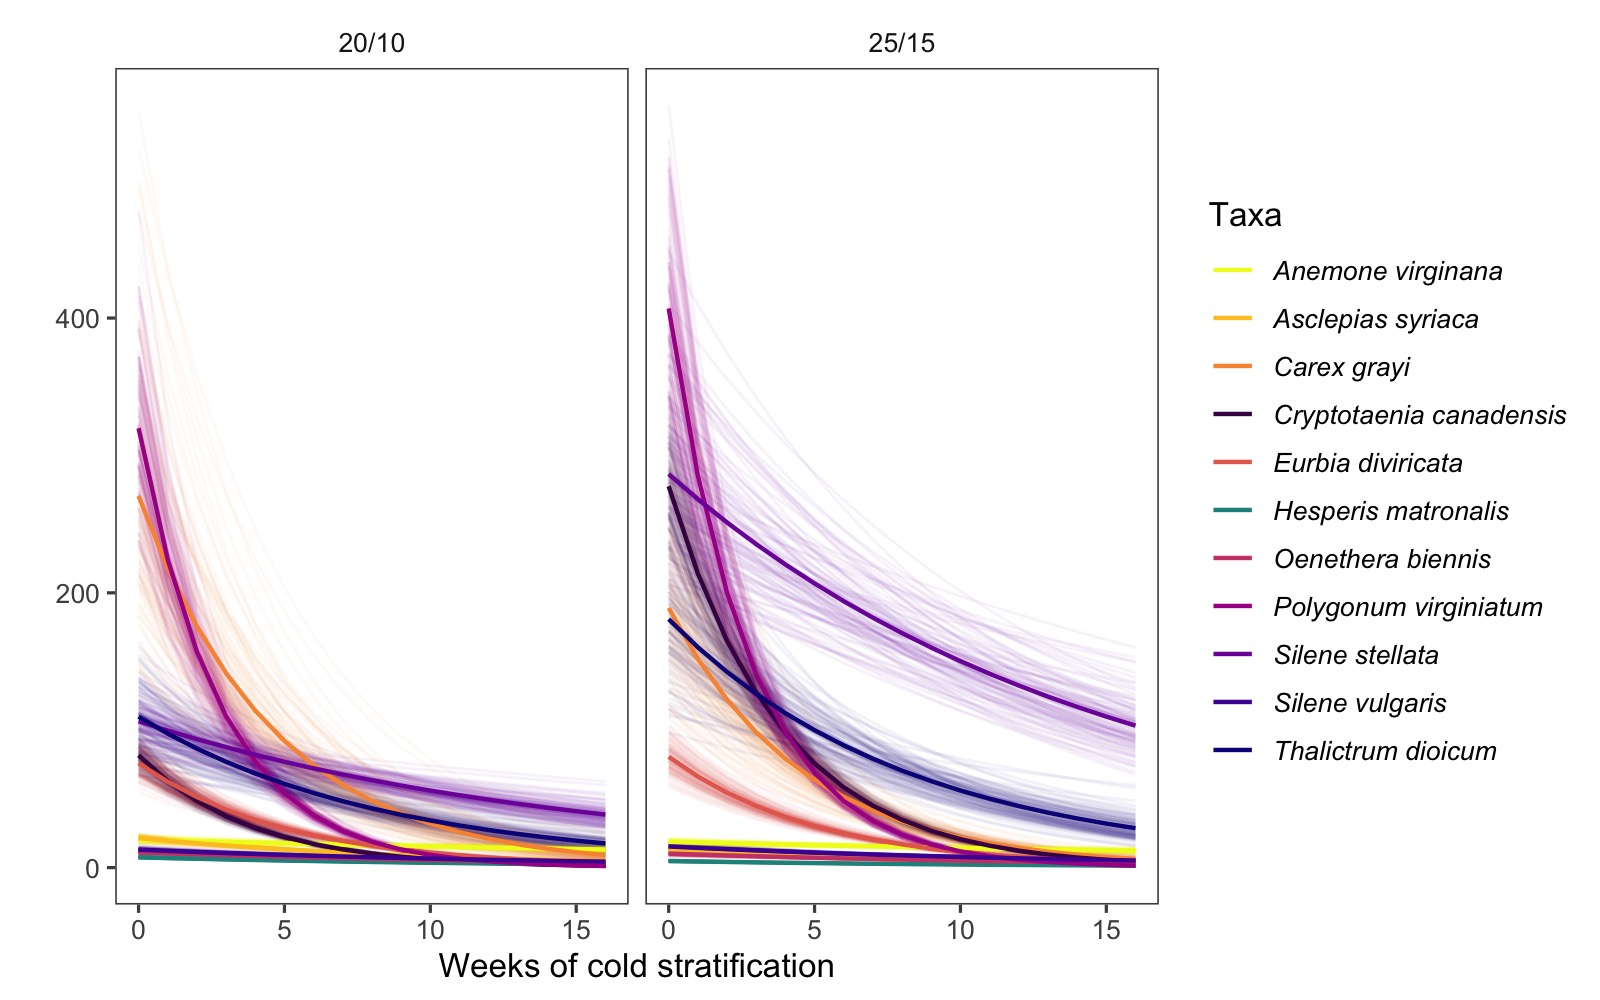
\includegraphics[width=\textwidth]{..//figure/AFTall.jpeg}
%   \caption{Estimated effect of weeks of cold stratification at 4$^\circ$C on the time to 50\% germination of 11 herbacious perennials under cool and warm (20/10$^\circ$C vs. 25/15$^\circ$C day/night) incubation conditions. The solid lines indicate the mean estimate, while lighter line indicate uncertainty.} 
%   \label{fig:AFTall}
%\end{figure}

\begin{figure}[hp]
    \centering
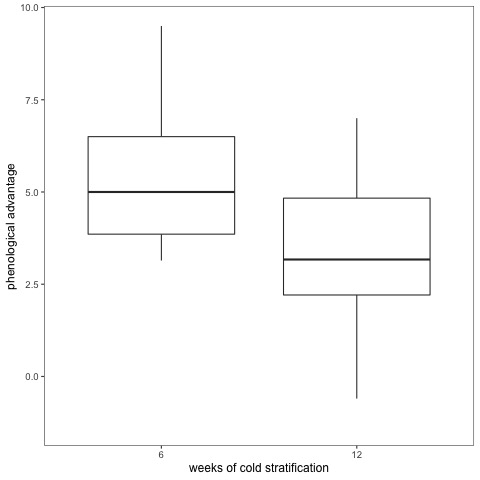
\includegraphics[width=.7\textwidth]{..//figure/priority_treat.jpeg}
   \caption{Differences in mean germination time (phenological advantage) between \textit{Hesperis matronalis} and \textit{Cryptotaenia canadensis} in each mixed-species pot under 6 and 12 weeks of cold stratification. Boxplots are based on raw data with middle bars indicating the median phenological advantage between the two species at each treatment level and the lower and upper hinges representing the 25\% and 75\% quantiles respectively} 
   \label{fig:MGTsup}
\end{figure}

\pagebreak
\section*{Co-occurence of focal species}

To assess how frequently our focal species co-occur in nature, we queried\linelabel{occ1a}  a recently published database of more than 80,000 plant community survey plots conducted through federal and state agencies \citep{Petri:2022tp} and found that of the 136 research plots invaded by \emph{H. matronalis}, \emph{C. canadensis} was present at 24\%, suggesting interactions between these species in the wild are common, meeting our second criteria of species\linelabel{occ2a} selection. To put this number in context, we compared it with all other native forb species (Tab. \ref{tab:occoverlap}), and found this value is quite high (9th highest) compared to all other native forb species co-occurrence rates (with none above 50\%). %emwmar31 -- check my edits here and add table ref. 


\section*{Measures of germination speed}
There are important differences between time to 50\% germination (t50) and mean germination time (MGT) that make one or the other more appropriate for the two types of experiments we ran. t50 is an estimate of the time to 50\% germination of all seeds planted, while mean germinating time (MGT) is a measure of the time to 50\% germination of only individuals that actually germinated \citep{Soltani:2015aa}. In comparative germination assays, t50 is considered a better metric because it standardizes phenological estimates across variable germination fractions. In our competition trials, we only wanted to estimate the phenology of individuals that germinated, so we used MGT as our measure of germination phenology. Because MGT is sensitive to the final germination fraction, it is not surprising the MGT measurements in the competition trials  were lower than the t50 estimates in the germination assays.

\bibliography{..///refs/germination.bib}

\end{document}
